\documentclass[x11names, svgnames]{beamer}
\usepackage{listings}

\usetheme{sbi}

\title{Galaxy for linking bisulfite sequencing with RNA sequencing \textendash\ Introduction to sequencing data analysis}
\author{Markus Wolfien, Andrea Bagnacani, Olaf Wolkenhauer}

\definecolor{Gray}{gray}{0.85}
\newcommand{\eg}{\textit{e}.\textit{g}.$\,\,$}

\begin{document}


%
% title
%
\frame[noframenumbering,plain]{\maketitle}



%
% outline
%
\newcommand{\one}{Who are we?}
\newcommand{\two}{Gene expression}
\newcommand{\three}{Techniques to measure gene expression}
\newcommand{\four}{RNA Sequencing (RNA-Seq)}
\newcommand{\five}{Tools and materials}
\begin{frame}
  \frametitle{Outline}
  \begin{itemize}
    \itemsep1em
    \item \one
    \item \two
    \item \three
    \item \four
    \item \five
  \end{itemize}
\end{frame}



%
%
%
\begin{frame}
  \frametitle{\one}
  \begin{center}
    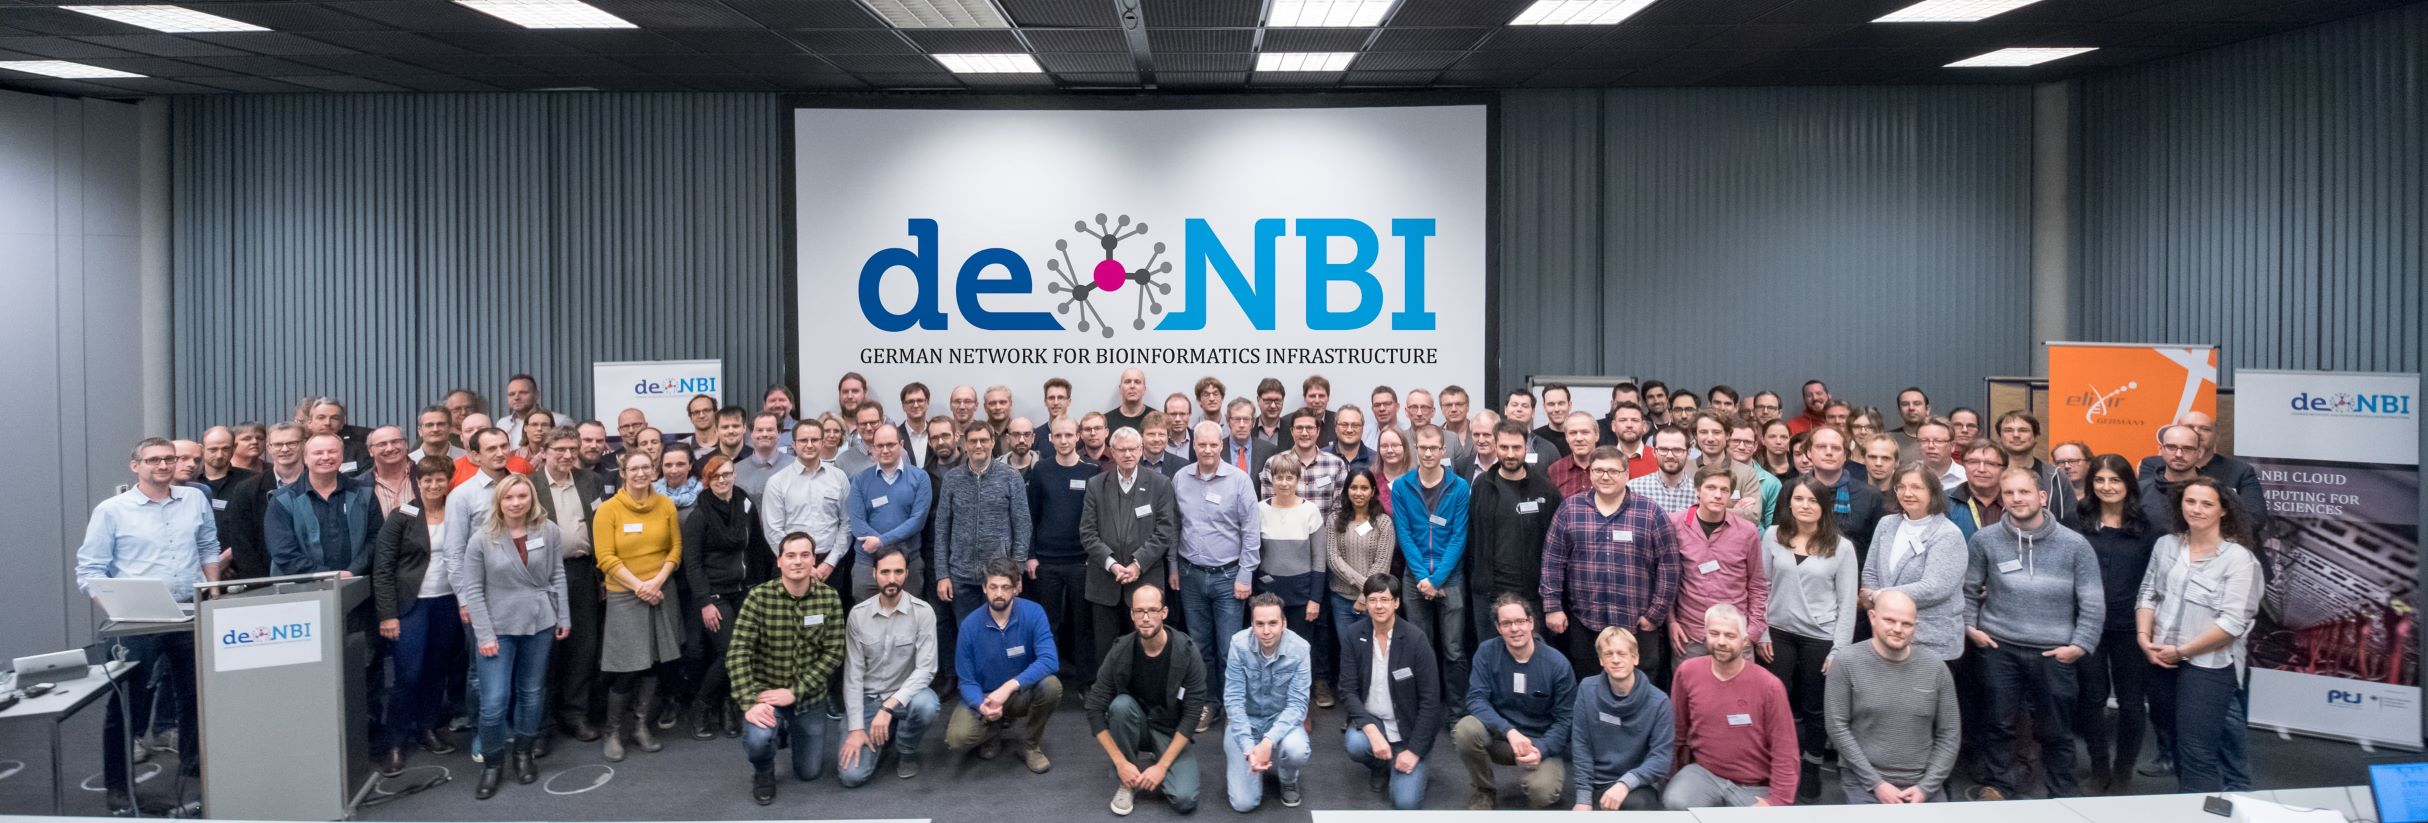
\includegraphics[scale=0.15]{images/people_denbi}
  \end{center}
  \begin{center}
    \footnotesize{\href{https://denbi.de}{\textcolor{gray}{https://denbi.de}}}
  \end{center}
  \begin{center}
    \small{
  The \textit{German Network for Bioinformatics Infrastructure} - \textbf{de.NBI} consists of eight service units that provide distinct bioinformatics services according to their areas of scientific expertise and their bioinformatics resources. The units complement each other in terms of thematic priorities, implementing user services in different areas of Life Sciences research and in industry. The services are complemented by comprehensive training activities.}
  \end{center}
\end{frame}
\begin{frame}
  \frametitle{\one}
  \begin{center}
    
\includegraphics[scale=0.3]{images/logo_destair}
  \end{center}
  \begin{center}
    \footnotesize{\href{https://destair.bioinf.uni-leipzig.de}{\textcolor{gray}{https://destair.bioinf.uni-leipzig.de}}}
  \end{center}
  \begin{center}
    \vspace{2em}
    \small{
    The \textit{Structured Analysis and Integration of RNA-Seq experiments} - \textbf{de.STAIR} provides comprehensive analyses of RNA-Seq experiments as a service. To bring ease of use, reproducibility, and accessibility for the developed approaches and services, we provide dedicated workshops, training programs and screen casts for bioinformaticians and other life scientists.}
  \end{center}
\end{frame}
\begin{frame}
  \frametitle{\one}
  \begin{center}
    Who are you? :)
  \end{center}
\end{frame}



%
%
%
\begin{frame}
  \frametitle{\two}
  \parbox{\linewidth}{\textbf{Gene expression} is the process by which genes in a DNA strand synthesise \textit{functional gene products}.\newline}
  \parbox{\linewidth}{Here, functional gene products can be Proteins or regulatory RNAs.\newline}
  \begin{itemize}
    \itemsep1em
    \item ...on the production side, proteins determine a cell's function, and therefore a cell's differentiations
    \item ...on the regulatory side, regulatory RNAs shape the amount of proteins, providing the cell control over its structure and function
  \end{itemize}
\end{frame}



%
%
%
\begin{frame}
  \frametitle{\three}
  \textbf{Northern blot} detects transcribed mRNAs within a mixture of RNA molecules in a sample.
  \begin{center}
    \vspace{-1.0em}
    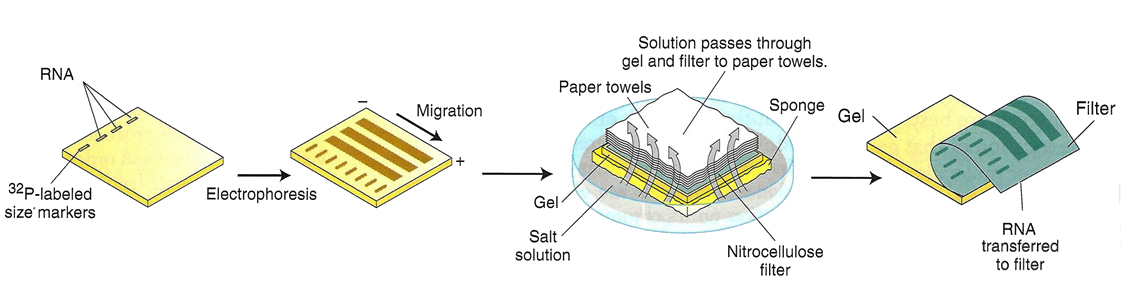
\includegraphics[scale=0.28]{images/wiki_northern_blot_1}
  \end{center}
  \begin{center}
    \vspace{-1.0em}
    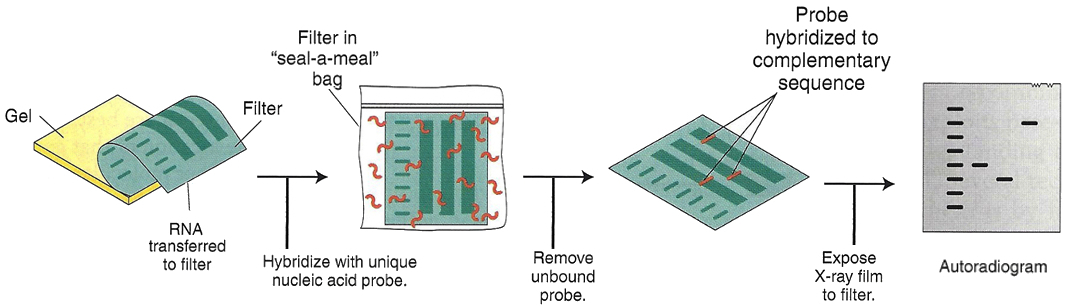
\includegraphics[scale=0.28]{images/wiki_northern_blot_2}
  \end{center}
\end{frame}

\begin{frame}
  \frametitle{\three}
  Northern blot procedure:\newline
  \begin{itemize}
    \item RNA backbone has phosphates (negatively charged)
    \item By applying current to the gel, RNAs migrate towards the positive end, separating by size
    \item RNA molecules are transfered (blotted) from the gel to a membrane
    \item RNA molecules are denaturated to loose their 3D structures
    \item Probes (fluorescent or radioactive) are washed against the membrane
    \item Probes bind against the complementar RNA molecule
    \item Exceeding probes are washed off. The ones bound to RNAs, provide a visual display of the presence of the target RNA molecules
  \end{itemize}
\end{frame}

\begin{frame}
  \frametitle{\three}
  \textbf{Northern blot is quantitatively inaccurate for small samples}.\newline\newline
  \begin{minipage}{0.50\textwidth}
    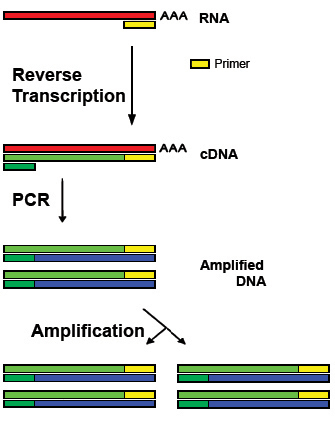
\includegraphics[scale=0.36]{images/wiki_rt-pcr}
    \begin{center}
      \vspace{-0.5em}
      \href{https://doi.org/10.1677/jme.0.0250169}{\textcolor{gray}{\tiny{Bustin. Journal of Molecular Endocrinology 2000}}}
    \end{center}
  \end{minipage}
  \begin{minipage}{0.45\textwidth}
  A solution to the inaccuracies coming from the availability of small RNA samples, has been provided by the \textbf{Reverse Transcription Polimerase Chain Reaction} (\textbf{RT-PCR}).\newline
    \begin{itemize}
      \small{
        \vspace{-1.0em}
        \item RT-PCR amplifies expressed genes by reverse transcribing the RNA of interest into its DNA complement
        \item This is achieved using reverse transcriptase
      }
    \end{itemize}
  \end{minipage}
\end{frame}

\begin{frame}
  \frametitle{\three}
  But \textbf{Northern blot and RT-PCR are very time consuming}!\newline
  \newline
  \parbox{\linewidth}{\textbf{Microarray} chips represent a step forward in the automation and measurement of gene expression levels, and are able to assess it for large numbers of genes in parallel.}
  \begin{center}
    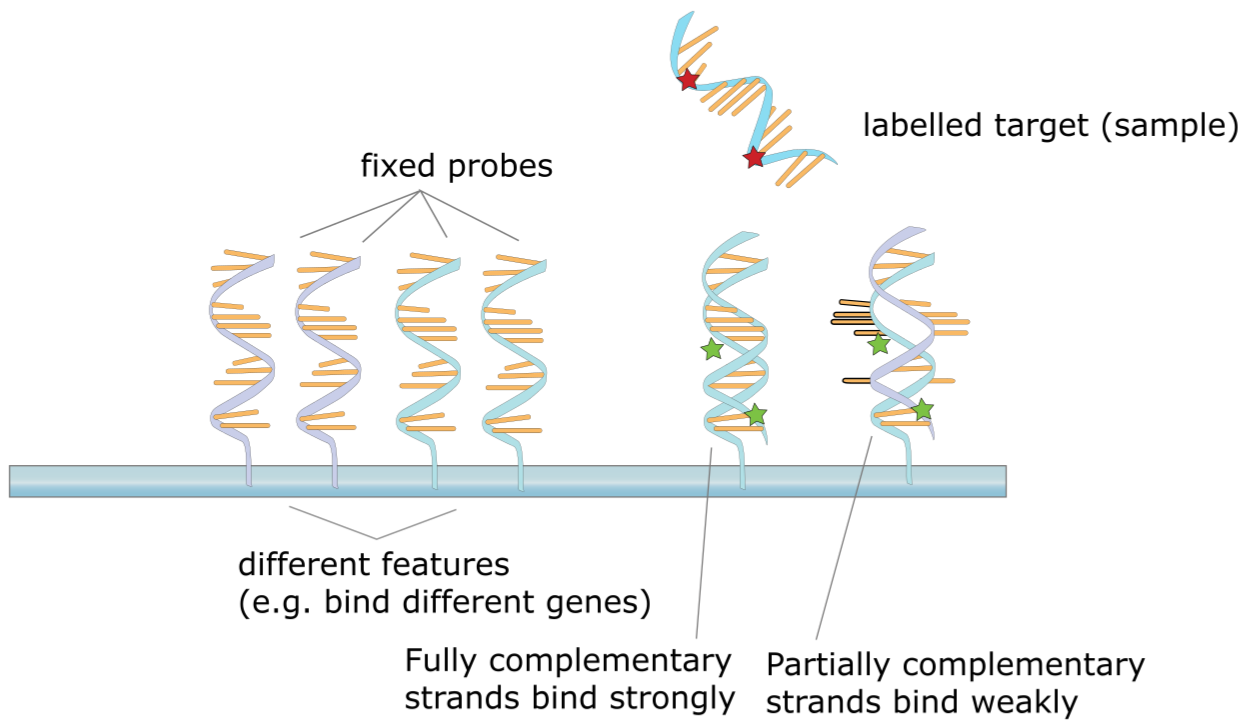
\includegraphics[scale=0.8]{images/wiki_hybridisation}
  \end{center}
\end{frame}

\begin{frame}
  \frametitle{\three}
  Microarray procedure:\newline
  \begin{center}
    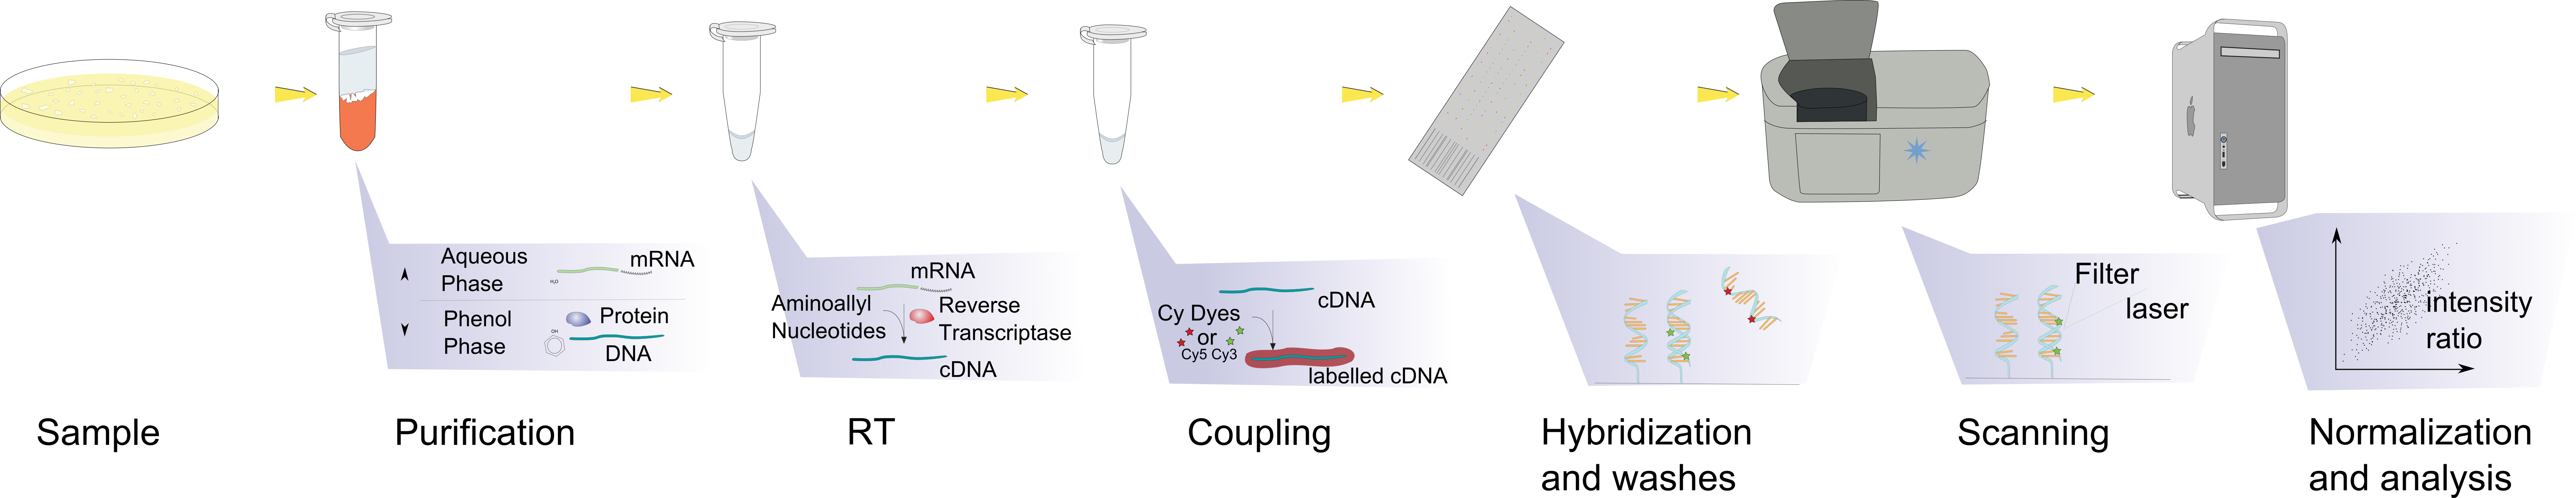
\includegraphics[scale=0.15]{images/wiki_microarray}
  \end{center}
  \begin{itemize}
    \item They consist of a surface organised into wells. Each well has \textit{probes} i.e. known sequences of DNA
    \item Targets are labelled with a fluorophore that produces a chemoluminescence
    \item Targets \textit{hybridise} to their corresponding probes, binding tightly or weakly
    \item The surface is washed to get rid of the weakly bound targets, and then scanned to analyse the chemoluminescence within each well
  \end{itemize}
\end{frame}

\begin{frame}
  \frametitle{\three}
  However, \textbf{microarray data is difficult to compare and reuse}:\newline
  \begin{itemize}
    \itemsep1em
    \item Lack of standardization in platform production
    \item Protocol diversity
    \item Multiple image analysis approaches
  \end{itemize}
  \vspace{2.0em}
  $\implies$ Interoperability problem
\end{frame}

\begin{frame}
  \frametitle{\three}
  \parbox{\linewidth}{\textbf{NGS enables massively parallel sequencing of DNA fragments, and can be used to analyse gene expression}.}
  \begin{center}
    \hspace*{-2.5em}
    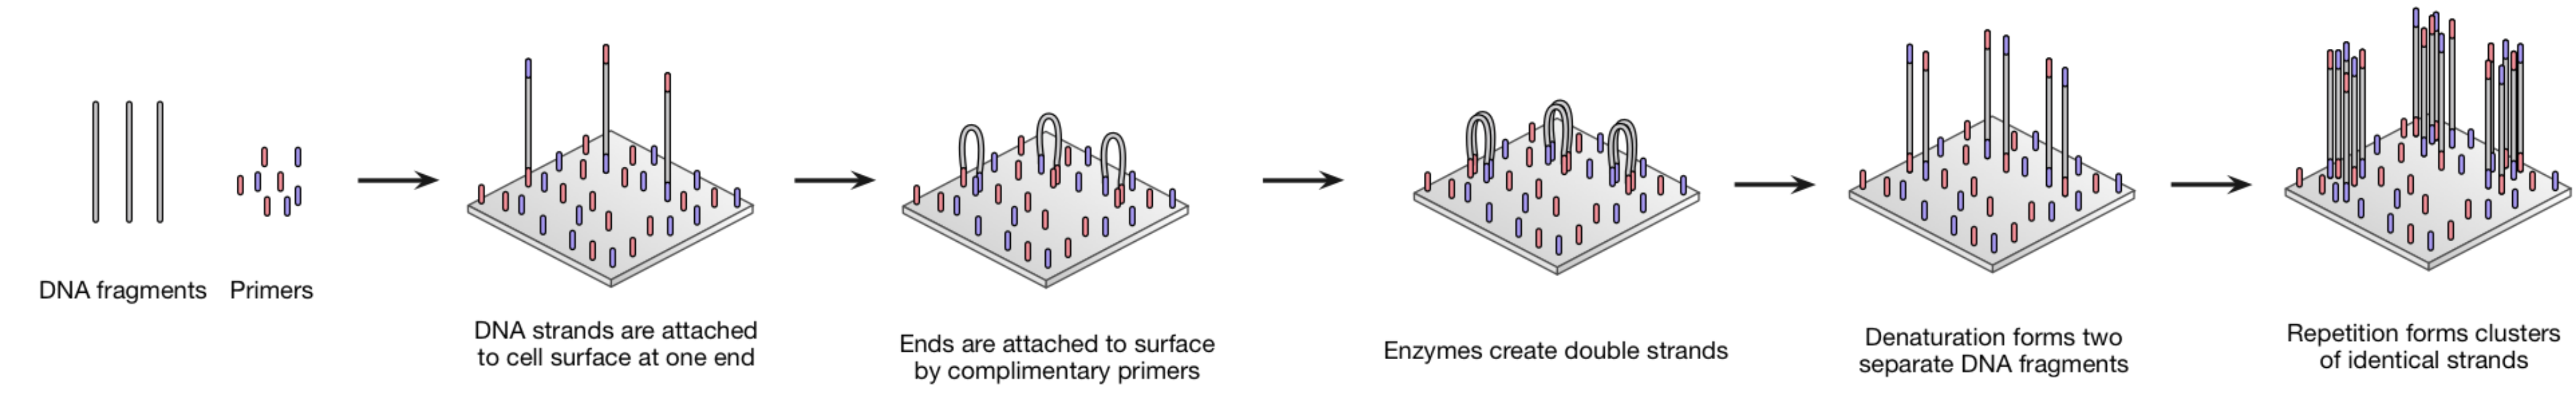
\includegraphics[scale=0.3]{images/atdbio_bridging_pcr}
  \end{center}
  \begin{itemize}
    \item DNA is isolated, fragmented, and primed on both ends
    \item Fragments are hybridised to the surface, where PCR amplifies them, creating clusters of DNA fragments
    \item Nucleotides are incorporated one after the other. They have a fluorophore and a terminator sequence to: 1) emit light, 2) prevent multiple binding
    \item The platform scans for the luminescence, then washes away fluorophores and terminator sequences
  \end{itemize}
\end{frame}

\begin{frame}
  \frametitle{\three}
  \begin{columns}[T]
    \begin{column}{0.5\textwidth}
      \begin{center}
        \vspace{-2em}
        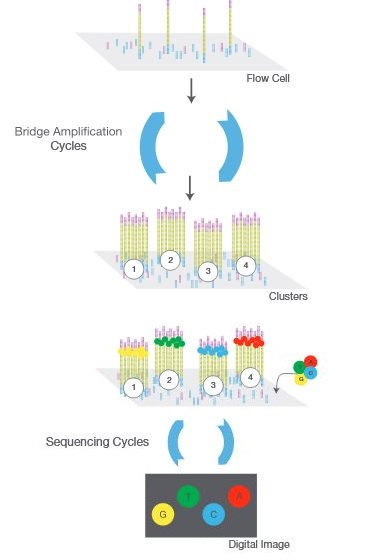
\includegraphics[scale=0.55]{images/illumina_sequencing}
      \end{center}
    \end{column}
    \begin{column}{0.5\textwidth}
      \begin{center}
        \vspace{-1em}
        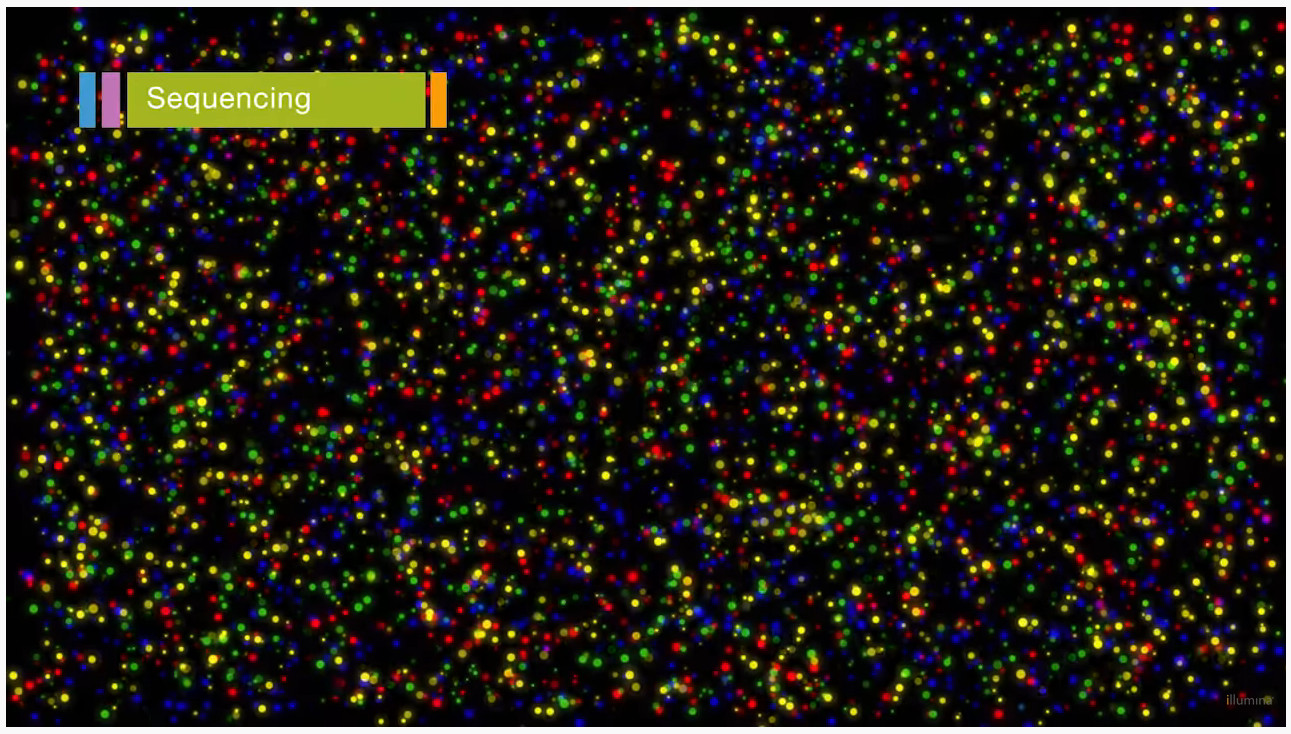
\includegraphics[scale=0.15]{images/illumina_video}
      \end{center}
      \begin{center}
        \tiny{\href{https://www.youtube.com/watch?v=fCd6B5HRaZ8}{\textcolor{gray}{https://www.youtube.com/watch?v=fCd6B5HRaZ8}}}
      \end{center}
      \vspace{4em}
      \footnotesize{
        \hfill\href{https://www.well.ox.ac.uk/ogc/sequencing-quality-monitoring-run/}{\textcolor{gray}{Oxford Genomics Centre, 2017}}
      }
      \vspace{6em}
      \footnotesize{
        \hfill\href{https://emea.illumina.com/content/dam/illumina-marketing/documents/products/other/ivf-reproductive-genetic-health-ngs-primer-1570-2015-012.pdf}{\textcolor{gray}{Illumina, 2015}}
      }
    \end{column}
  \end{columns}
\end{frame}

\begin{frame}
  \frametitle{\three}
  \textbf{The more the readout process progresses, the less confident the reads become}. This is due to the removal of the fluorescent dye, which becomes progressively difficult, leaving background noise to the further readouts.\newline
  \vspace{2em}
  \begin{minipage}{0.45\textwidth}
    \hspace*{-1.2em}
    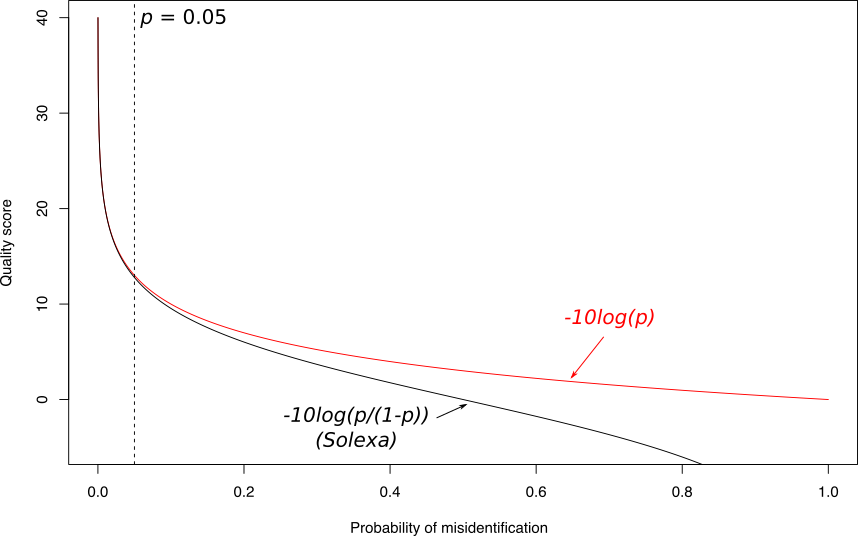
\includegraphics[scale=0.22]{images/quality_score}
  \end{minipage}
  \begin{minipage}{0.50\textwidth}
    \hspace*{1.3em}
    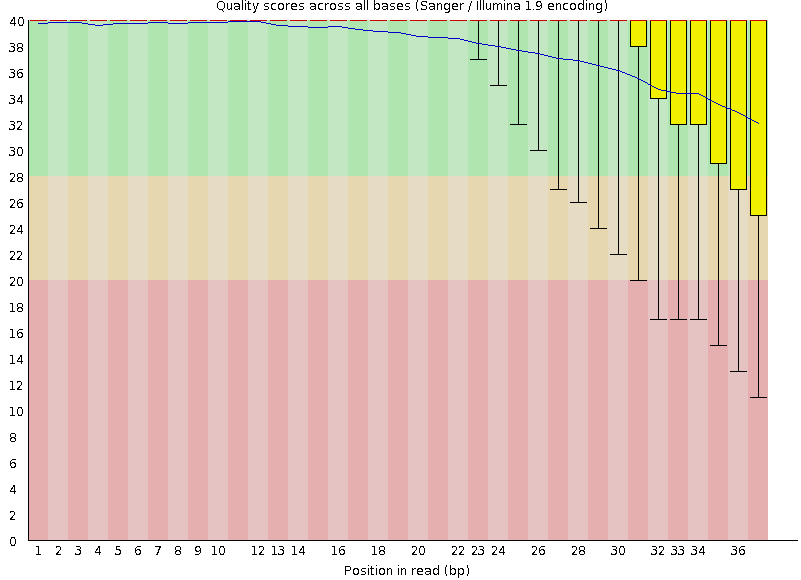
\includegraphics[scale=0.2]{images/per_base_sequence_quality_good}
  \end{minipage}
\end{frame}

\begin{frame}
  \frametitle{\three}
  The decrease of sequencing costs is met with an increased effort in data processing $\implies$ Increased need of Bioinformatics expertise.
  \begin{center}
    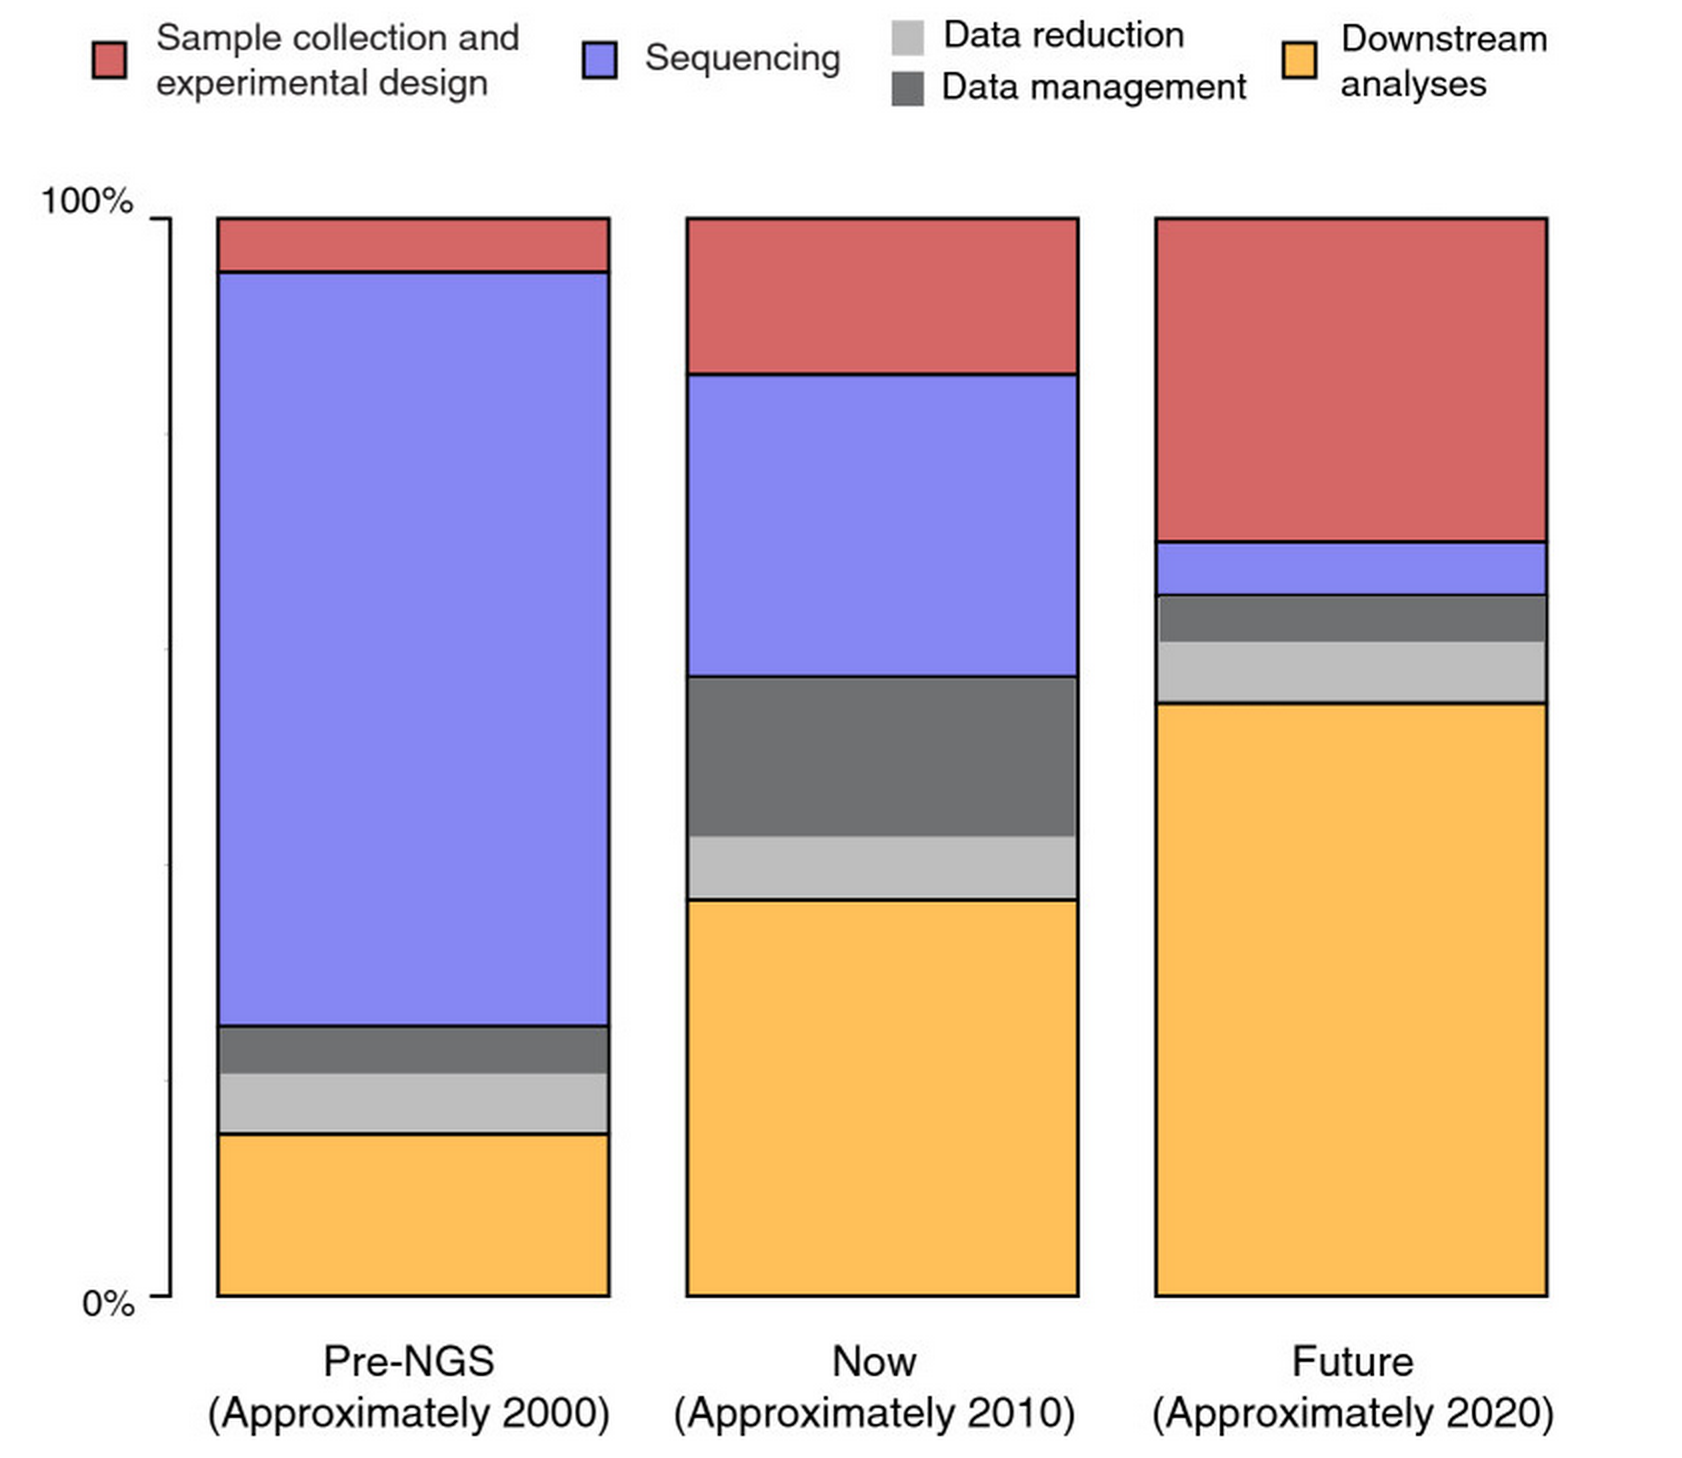
\includegraphics[scale=0.11]{images/sequencing_cost}
  \end{center}
  \begin{center}
    \vspace{-0.5em}
    \footnotesize{\href{https://doi.org/10.1186/gb-2011-12-8-125}{\textcolor{gray}{Sboner et al., Genome Biology 2011}}}
  \end{center}
\end{frame}



%
%
%
\begin{frame}
  \frametitle{\four}
  \begin{center}
  RNA-Seq is able to identify thousands of differentially expressed genes, tens of thousands of differentially expressed gene isoforms and can detect mutations and germline variations for hundreds to thousands of expressed genetic variants, as well as detecting chimeric gene fusions, transcript isoforms and splice variants.
  \end{center}
  \begin{center}
    \vspace{2em}
    \footnotesize{\href{https://doi.org/10.1038/nrg2484}{\textcolor{gray}{Wang, Nature 2009}}}
  \end{center}
\end{frame}
\begin{frame}
  \frametitle{\four}
  \begin{center}
    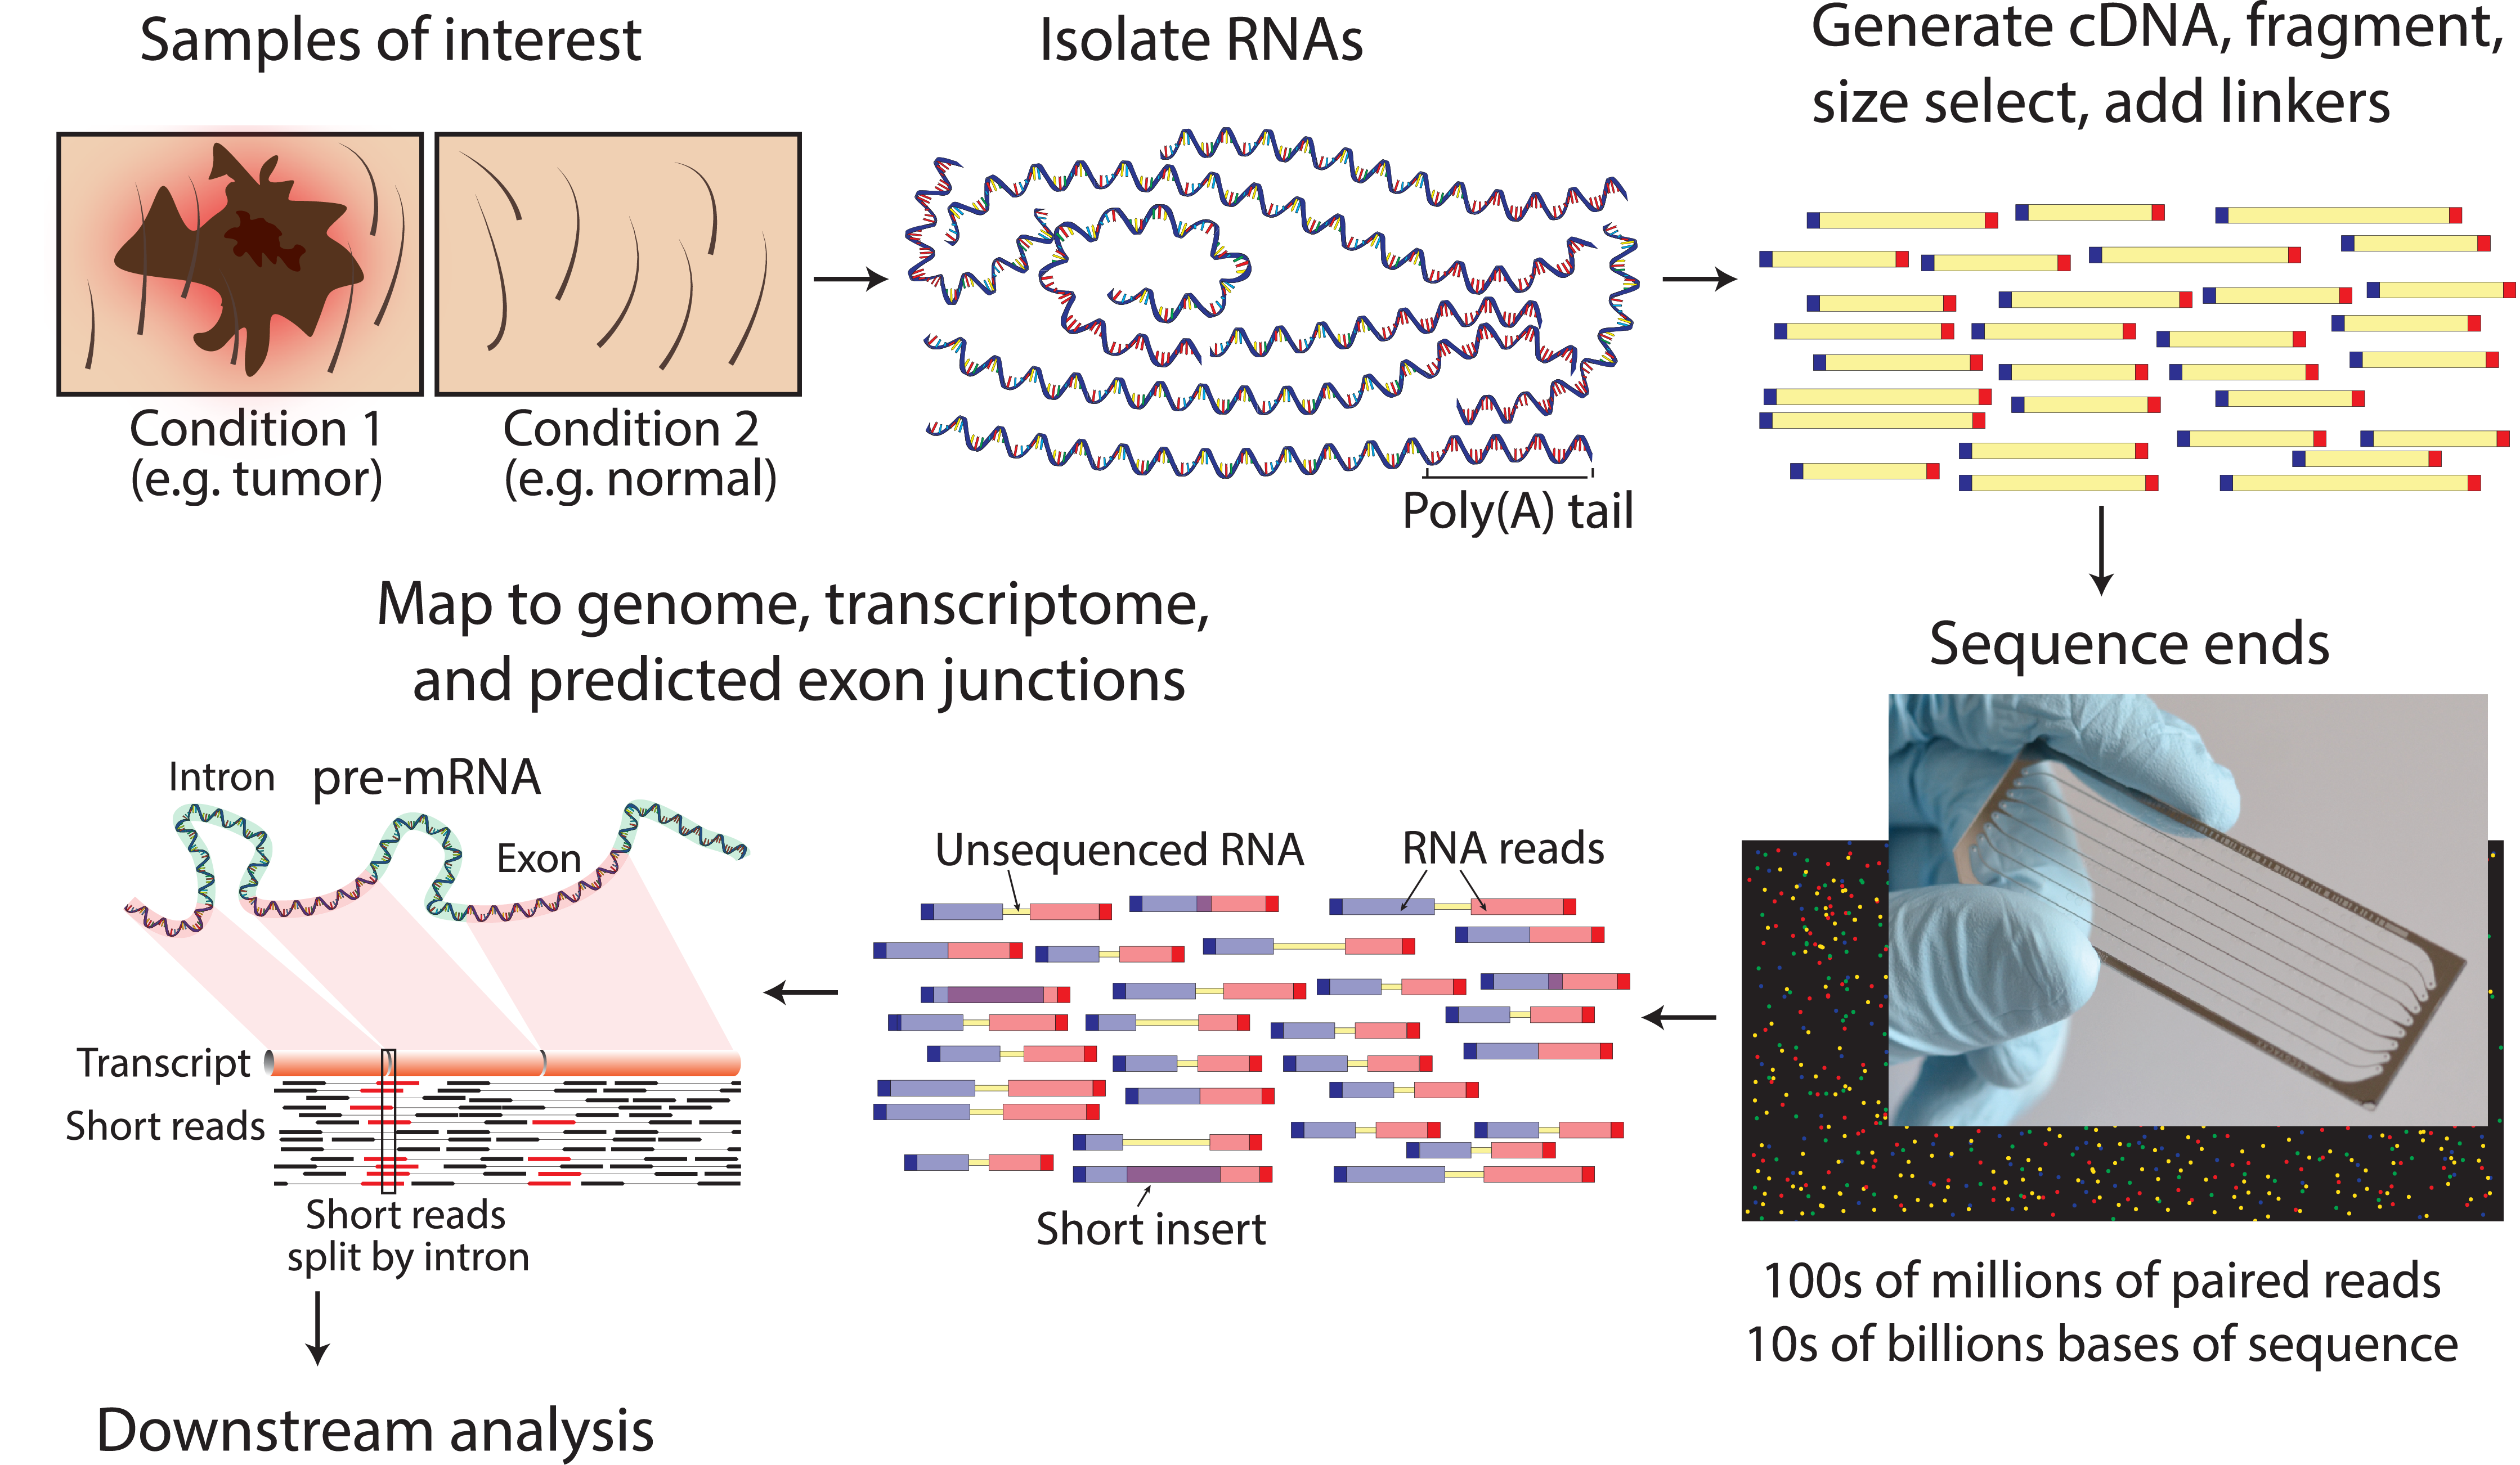
\includegraphics[scale=0.55]{images/griffith-plos}
  \end{center}
  \begin{center}
    \vspace{1.5em}
    \footnotesize{\href{https://doi.org/10.1371/journal.pcbi.1004393}{\textcolor{gray}{Griffith et al., PLOS 2015}}}
  \end{center}
\end{frame}

\begin{frame}
  \frametitle{\four}
  \textbf{No unique way of carrying out any data analysis workflow}.\newline
  \newline
  RNA-Seq workflow:
  \begin{center}
    
\includegraphics[scale=0.2]{images/workflow-rna-seq}
    \vspace{1em}
  \end{center}
  Tools:
  \begin{center}
    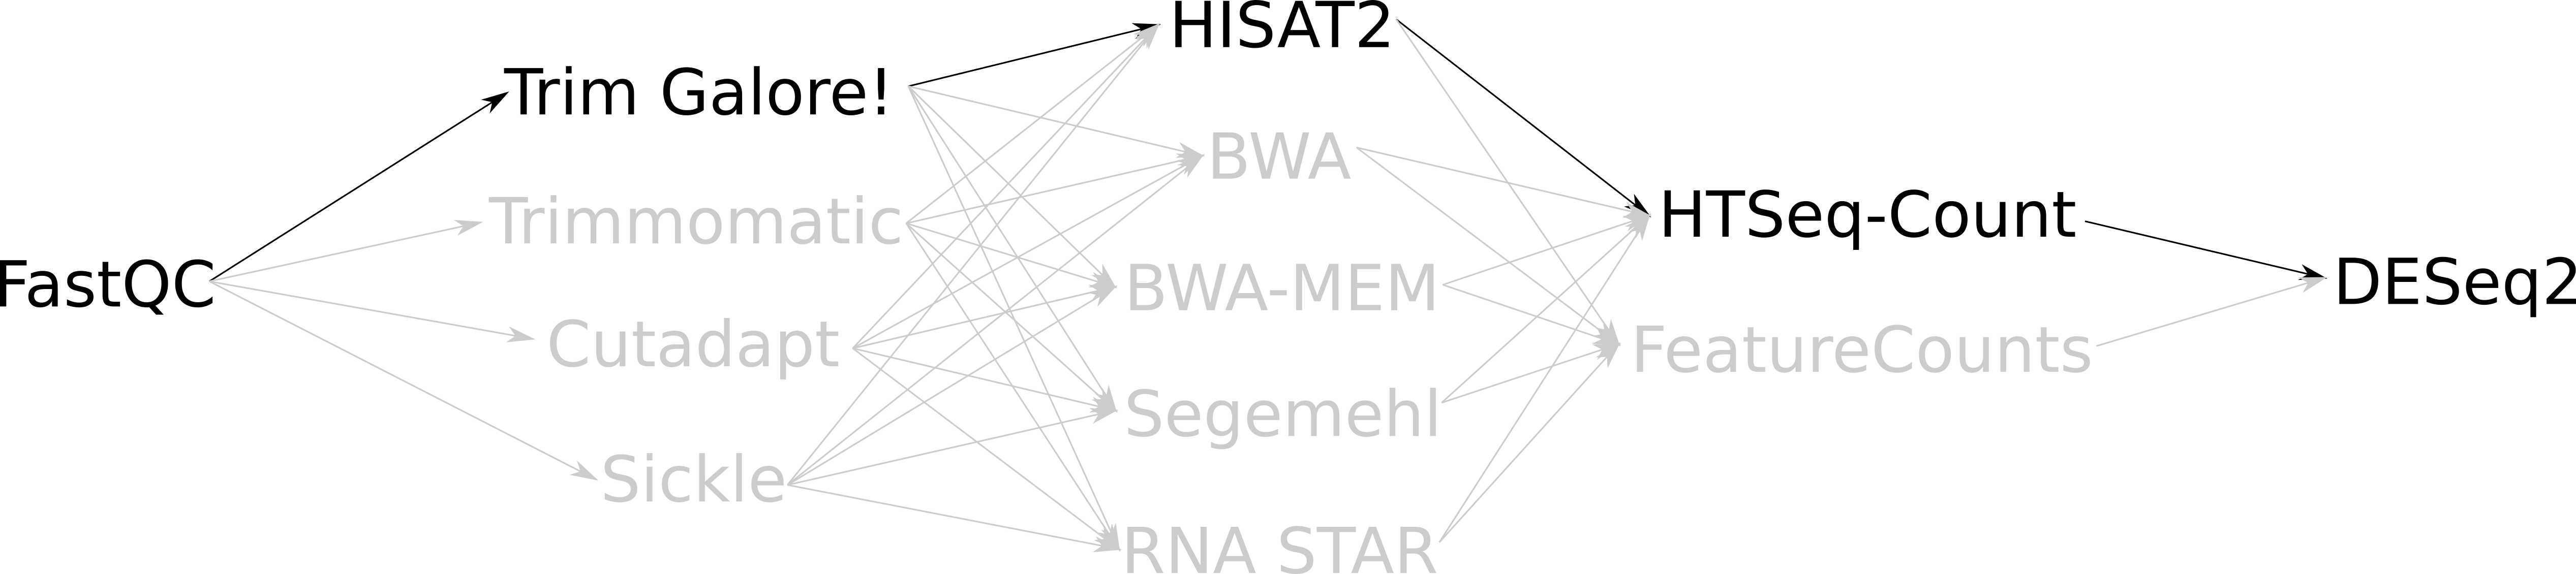
\includegraphics[scale=0.2]{images/workflow-rna-seq-tools-preferred}
    \vspace{1em}
  \end{center}
  Each tool has its own software dependencies!
\end{frame}


%
%
%
\begin{frame}
  \frametitle{\five}
  \begin{center}
    \vspace{-1em}
    
\includegraphics[scale=0.05]{images/logo_github}
  \end{center}
  \begin{center}
    \vspace{-1em}
    \footnotesize{\href{https://github.com/destairdenbi/trainings}{\textcolor{gray}{https://github.com/destairdenbi/trainings}}}
  \end{center}
  \begin{center}
    \vspace{1.5em}
    
\includegraphics[scale=0.05]{images/logo_galaxy}
  \end{center}
  \begin{center}
    \vspace{-1em}
    \footnotesize{\href{https://usegalaxy.eu}{\textcolor{gray}{https://usegalaxy.eu}}}
  \end{center}
  \begin{center}
    \vspace{1.5em}
    
\includegraphics[scale=0.08]{images/logo_gtn}
  \end{center}
  \begin{center}
    \vspace{-1em}
    \footnotesize{\href{https://galaxyproject.github.io/training-material/}{\textcolor{gray}{https://galaxyproject.github.io/training-material/}}}
  \end{center}
\end{frame}

\end{document}
